\chapter{Panoramica tecnica}

L'utilizzo di varie tecniche di protezione hanno reso sempre più
difficile lo sfruttamento di errori nell'esecuzione di un programma al
fine di prenderne il controllo. Questo capitolo introduce brevemente
alcune di queste tecniche e analizza con quali metodi è possibile
eluderle. Anche se alcuni concetti sono indipendenti dall'architettura
e dal sistema operativo si tratterà esclusivamente di come queste
tecniche sono implementate in ambiente GNU/Linux, su architettura x86
e x86-64. Nella prima parte di si parlerà brevemente dei principali
meccanismi con i quali il sistema operativo, partendo dalle
informazioni presenti all'interno di un file oggetto eseguibile, crea
una rappresentazione dinamica del programma, detta \emph{immagine del
  processo}. Nella seconda parte invece verranno analizzate alcune
tecniche di exploit.

\section{Creazione dell'immagine di un processo}

Su sistemi operativi GNU/Linux per la rappresentazione statica dei
programmi viene utilizzato il formato ELF.  ELF (Executable and
Linkable Format) può rappresentare tre tipi di file oggetto:

\begin{itemize}
  \item \emph{file oggetto rilocabile}: contiene dati e codice che
    vengono collegati ad altri file oggetto al fine di ottenere un
    \emph{file oggetto eseguibile} o un \emph{file oggetto condiviso}

  \item \emph{file oggetto eseguibile}: è la rappresentazione statica
    di un programma che può essere eseguito, questo file ha le
    informazioni necessarie affinché il sistema operativo crei la sua
    immagine di processo

  \item \emph{file oggetto condiviso} che contiene codice e dati
    adatti per essere collegati (nel processo di linking) in due
    contesti differenti. Può essere infatti utilizzato sia in fase di
    building insieme ad altri file oggetto rilocabili o file oggetto
    condivisi (\emph{linking statico}) per creare altri file oggetto,
    oppure può essere collegato in fase di creazione dell'immagine del
    processo di un file oggetto eseguibile (\emph{linking dinamico}).

\end{itemize}

Il formato ELF può contenere sia le informazioni necessarie per
processi relativi alla fase di creazione di diversi file oggetto a
partire da file sorgente (in particolare informazioni necessarie per
la fase di linking), sia relativamente allo scopo della creazione
dell'immagine di un processo a partire da un file oggetto
eseguibile. Anche le strutture dati all'interno dell'ELF afferenti di
questi due ``punti di vista'' sono diverse, e, a seconda della
tipologia del file oggetto alcune delle strutture dati possono non
essere presenti. Essendo più rilevante ai fini del nostro lavoro ci
concentreremo principalmente sulle strutture dati rilevanti nelle
operazioni di creazione dell'immagine del processo e nelle procedure
di dynamic linking, ovvero nel processo con il quale si rendono
fruibili all'eseguibile i metodi esposti da una libreria condivisa a
tempo di esecuzione.

\subsection{Program Header Table}
\label{sec:plt}

L'ELF header (che è l'unica struttura dati che ha una posizione fissa
all'interno del file) funge da una sorta di mappa, e ci consente di
localizzare tutte le altre strutture dati presenti nel file.

Tra queste vi è la \emph{Program Header Table}. La Program Header
Table è un array di strutture, ognuna delle quali contiene o
informazioni su come costruire un segmento della memoria dell'immagine
di un processo o informazioni per la preparazione dell'immagine
stessa. Un elemento all'interno della Program Header Table (su
un'architettura a 32bit) è rappresentata dalla seguente struttura C:

\begin{lstlisting}[caption=Program Header Table entry]
typedef struct {
  uint32_t   p_type;
  Elf32_Off  p_offset;
  Elf32_Addr p_vaddr;
  Elf32_Addr p_paddr;
  uint32_t   p_filesz;
  uint32_t   p_memsz;
  uint32_t   p_flags;
  uint32_t   p_align;
} Elf32_Phdr;
\end{lstlisting}

La struttura relativa ad un'architettura a 64bit è pressoché identica,
l'unica differenza sta nella posizione degli attributi.  L'attributo
\lstinline{ptype} indica il tipo di entry. Per il nostro scopo ci
limiteremo a descrivere le entry di tipo \lstinline{PT_LOAD},
\lstinline{PT_INTERPETER} e \lstinline{PT_DYNAMIC}. Le entry di tipo
\lstinline{PT_LOAD} rappresentano informazioni su un segmento da
caricare in memoria. Il campo \lstinline{p_offset} e
\lstinline{p_filesz} indicano rispettivamente l'offset e la sua
grandezza all'interno del file. \lstinline{p_vaddr} e
\lstinline{p_memsz} invece indicano rispettivamente il base address
nel quale caricare in memoria il segmento e la dimensione che avrà in
memoria (che potrebbe essere più grande rispetto a quella sul
file). \lstinline{p_flags} è molto rilevante per il nostro lavoro e
indica con quali flags il segmento andrà ad essere caricato in memoria
ovvero se il segmento sarà o meno scrivibile, leggibile e/o
eseguibile. Tuttavia nel caso il segmento contenga codice compilato
affinché risulti indipendente dall'indirizzo base nel quale risiede in
memoria, il campo \lstinline{p_vaddr} potrebbe essere nullo e la
posizione del segmento in memoria potrebbe essere casualizzata.

La voce all'interno della Program Header Table con il tipo
\lstinline{PT_INTERP} invece contiene una stringa che rappresenta il
percorso di un file oggetto eseguibile o condiviso all'interno del
filesystem, detto interprete. Il sistema operativo crea l'immagine del
processo dell'interprete, dandogli il controllo. Sarà compito poi
dell'interprete creare l'immagine del processo necessaria
all'esecuzione dell'eseguibile. Affinché questo possa accadere
l'interprete avrà accesso alle informazioni presenti nel file
principale. Normalmente l'interprete è costituito da codice
indipendente dalla posizione nella quale viene caricato, che viene
casualizzata evitando conflitti tra gli spazi di memoria utilizzati
dall'eseguibile principale e quelli dell'interprete stesso.

Quando viene creato del codice oggetto che utilizza delle librerie
dinamiche, il linker aggiunge alla Program Header Table un elemento di
tipo \lstinline{PT_INTERPRETER} con impostato come interprete il
\emph{dynamic linker}, che si occupa di trovare le librerie necessarie
all'eseguibile, caricarle in memoria, caricare in memoria i segmenti
dell'eseguibile, risolvere le relocation verso i simboli delle
librerie, e ridare poi controllo all'eseguibile stesso. Come vedremo
la risoluzione di un simbolo potrebbe essere rimandata fin quando non
sia realmente necessario. A supporto di questi processi troviamo
alcune strutture dati, anch'esse aggiunte al file oggetto eseguibile
durante la fase di linking. Queste strutture risiedono all'interno di
segmenti che vengono caricati in memoria, e sono quindi disponibili
durante l'esecuzione del programma. Informazioni su dove trovare
queste strutture dati possono essere ricavate attraverso un'altra
struttura dati del file ELF, la \emph{Section Header Table}, che è un
array di strutture che descrivono, per l'appunto, le parti che
compongono il file, dette sezioni. Tuttavia, anche se nel nostro
lavoro di tesi le sezioni vengono utilizzate per ottenere informazioni
sul binario esaminato, è da notare che esse non sono necessarie per un
file oggetto di tipo eseguibile. Un file oggetto infatti può essere
caricato esclusivamente con le informazioni presenti nella Program
Header Table (lo strumento sstrip\cite{sstrip} elimina appunto le
sezioni da un file eseguibile). Tuttavia è conveniente per scopi
illustrativi riferirsi alle strutture dati relative al processo di
dynamic linking riferendosi alle rispettive sezioni, che sono:

\begin{itemize}

  \item Una sezione \lstinline{.dynamic} che contiene gli indirizzi di
    altre strutture necessarie al processo di dynamic linking e la
    lista delle librerie necessarie all'esecuzione del file oggetto
    eseguibile

  \item Una sezione \lstinline{.hash} che contiene una tabella dei
    simboli

  \item Le sezioni \lstinline{.got} e \lstinline{.plt} contengono
    rispettivamente due tabelle: \emph{la Global Offset Table} e
    \emph{la Procedure Linkage Table}. Nelle sezioni successive
    vedremo come queste due strutture dati vengono utilizzate dal
    dynamic linker per risolvere i simboli e le chiamate a funzioni
    presenti nelle librerie dinamiche

\end{itemize}

\subsection{Global Offset Table e Procedure Linkage Table}
\label{sec:got}

Un programma che sia indipendente dalla posizione in cui viene
caricato in memoria non può contenere al suo interno indirizzi
assoluti. Le Global Offset Table (\lstinline{GOT}) contengono
indirizzi assoluti in un'area di memoria privata destinata ai dati,
non compromettendo quindi l'indipendenza del codice dalla posizione in
memoria (e quindi che sia condivisibile da più immagini di processo,
come nel caso di una libreria dinamica). Il linker, una volta creata
l'immagine di un processo, processa tutte le rilocazioni (strutture
dati che contengono informazioni per la risoluzione dei simboli) di
tipo \lstinline{R_386_GLOB_DAT} e per ognuna di esse calcola
l'indirizzo assoluto. Il linker conoscendo l'indirizzo di tutti i file
oggetto caricati in memoria ha tutte le informazioni necessarie per
calcolare il valore di questi indirizzi. Una volta calcolati il linker
inserisce i valori assoluti nei rispettivi elementi della
\lstinline{GOT}, permettendo all'eseguibile di accedervi attraverso
posizioni relative.

A noi interessa principalmente come la \lstinline{GOT} è coinvolta nel
momento in cui un file oggetto eseguibile esegue una chiamata ad una
funzione di una libreria dinamica, processo in cui è coinvolta anche
una seconda tabella, la Procedure Linkage Table (\lstinline{PLT}).

La \lstinline{PLT} redireziona chiamate a funzioni che utilizzano
indirizzi relativi a indirizzi assoluti calcolati a tempo
d'esecuzione. In fase di building di un eseguibile il linker fa in
modo che chiamate a funzioni presenti in librerie dinamiche vengano
direzionate a elementi della \lstinline{PLT}. Anche se la
\lstinline{PLT} risiede nel segmento di memoria destinato a contenere
il codice di un eseguibile, utilizza valori nella Global Offset Table,
non compromettendo così né l'indipendenza dalla posizione ne la
condivisibilità del codice. È compito del dynamic linker calcolare i
valori degli indirizzi della funzione chiamata e impostarli nei
relativi elementi della \lstinline{GOT}. Nella restante parte di
questa sezione andremo a descrivere come il dynamic linker utilizza
queste due tabelle per risolvere gli indirizzi, facendo riferimento
all'implementazione su un'architettura a 32bit. Tuttavia il concetto
principale resta pressoché invariato anche per un'architettura a
64bit. Nel listato \ref{cod:plt} è illustrata la struttura della \lstinline{PLT}.

\begin{lstlisting}[caption=Procedure linkage table, label=cod:plt]
.PLT0:
    pushl   got_plus_4
    jmp     *got_plus_8
    nop;    nop
    nop;    nop
.PLT1:
    jmp     *name1_in_GOT
    pushl   $offset
    jmp     .PLT0@PC
.PLT2:
    jmp     *name2_in_GOT
    pushl   $offset
    jmp     .PLT0@PC
    ...
    ...
\end{lstlisting}

La risoluzione dell'indirizzo può essere sommarizzata nei seguenti
punti:

\begin{itemize}
\item Quando viene creata l'immagine del processo i primi due valori
  nella GOT assumono valori particolari (spiegati di seguito)
\item Quando l'eseguibile esegue una chiamata di una funzione in una
  libreria dinamica il flusso del programma viene indirizzato nella
  \lstinline{PLT}. Nel nostro esempio viene chiamata la funzione
  \lstinline{name1}, che avrà come indirizzo di destinazione
  l'istruzione marcata dall'etichetta \lstinline{.PLT1}
\item Il programma a questo punto esegue un \lstinline{jmp}
  all'indirizzo contenuto nell'elemento nella GOT relativo a
  \lstinline{name1}. Al momento di caricamento del programma, a
  eccezione di casi particolari come descritto di seguito, questo
  elemento è impostato con il valore dell'istruzione successiva al
  \lstinline{jmp} stesso, cioè all'istruzione alla linea 7 del listato
  \ref{cod:plt}
\item Il codice a questo punto salva sullo stack l'offset all'interno
  della tabella delle rilocazioni che permette di individuare la
  rilocazione relativa al simbolo \lstinline{name1}. La rilocazione
  permette di ricavare sia l'elemento della \lstinline{GOT} relativo a
  quel simbolo che il nome del simbolo stesso, fornendo le
  informazioni necessarie al dynamic linker per capire quale simbolo è
  stato chiamato e qual è l'elemento da modificare nella
  \lstinline{GOT}.
\item A questo punto il programma salta al primo elemento della
  \lstinline{PLT} e, dopo aver salvato sullo stack il secondo elemento
  della \lstinline{GOT}, salta all'indirizzo contenuto nel terzo
  elemento della got, che dà il controllo al dynamic linker
\item Il dynamic linker esamina lo stack, controlla quale simbolo è
  stato chiamato, calcola l'indirizzo e imposta il valore
  nell'elemento relativo nella \lstinline{GOT}. In questo modo una
  seconda chiamata a \lstinline{name1} non causerà una seconda
  chiamata al linker ma salterà direttamente all'indirizzo corretto
\end{itemize}

\begin{figure}
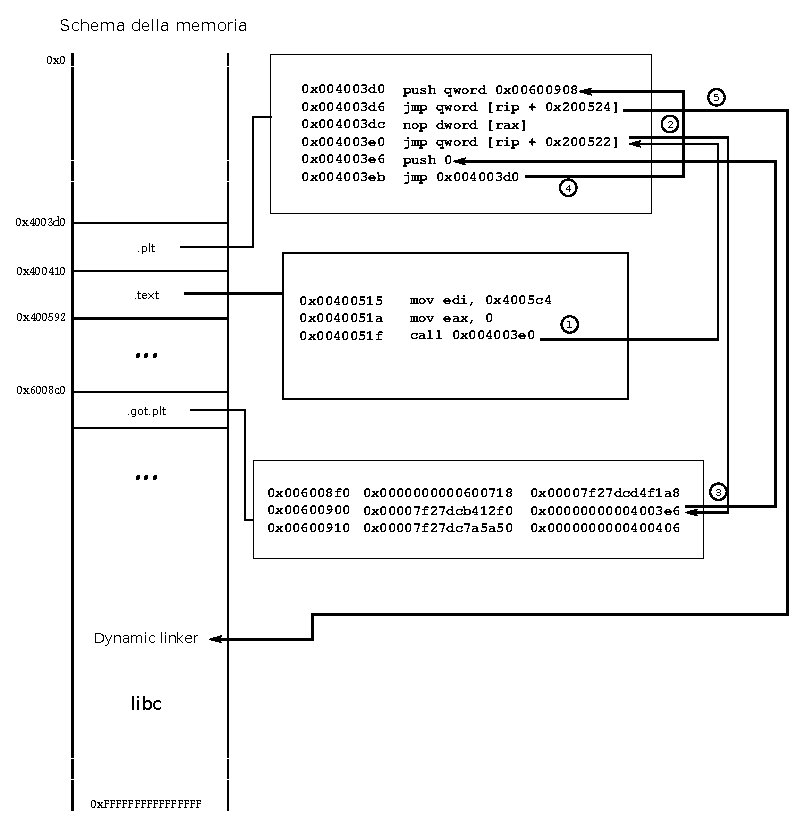
\includegraphics{plt_got_printf_diritta_prima} 
\caption{Fasi della chiamata ad una funzione di una libreria condivisa
  prima che nella GOT sia presente l'indirizzo della funzione}
\label{fig:got_plt_prima}
\end{figure}

\begin{figure}
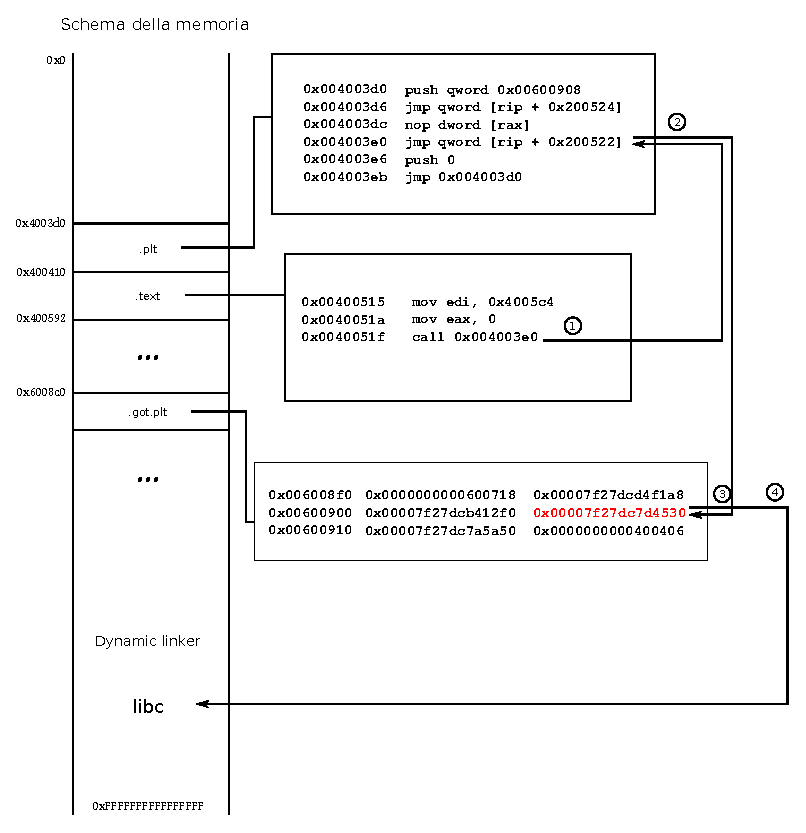
\includegraphics{plt_got_printf_diritta_seconda}
\caption{Fasi della chiamata ad una funzione di una libreria condivisa
  dopo che la GOT sia stata modificata con l'indirizzo della funzione
  dal dynamic linker}
\label{fig:got_plt_seconda}
\end{figure}


Le figure \ref{fig:got_plt_prima} e \ref{fig:got_plt_seconda}
riassumono i flussi di esecuzioni del programma illustrativo presente
nel listato \ref{cod:so} evidenziando le differenze tra la prima
chiamata alla funzione \lstinline{printf} e la seconda.

\begin{figure}
\begin{lstlisting}[language=c,label=cod:so,caption=codice del
    programma a cui fanno riferimento le figure
    \ref{fig:got_plt_prima} e \ref{fig:got_plt_seconda}]
#include <stdlib.h>
#include <stdio.h>

int main(int argc, char *argv[]) {
	printf("prima");
	printf("seconda");
	return 0;
}
\end{lstlisting}
\end{figure}

L'approccio appena descritto, nel quale gli indirizzi delle funzioni
vengono risolti solo al momento in cui vengono chiamate, viene
definito \emph{lazy binding}. Se invece il programma viene eseguito
con la variabile d'ambiente \lstinline{LD_BIND_NOW} impostata gli
indirizzi vengono tutti calcolati e scritti nella \lstinline{GOT} al
momento del caricamento dell'eseguibile. Questo comportamento avviene
anche quando si compila un eseguibile con l'opzione
\lstinline{RELRO}. Inoltre, in questo caso, una volta modificata la
\lstinline{GOT} viene resa non più scrivibile, in modo da mitigare
attacchi di tipo got patching.


\section{Return Oriented Programming}

Per mitigare classici attacchi di tipo stack-smashing sono state
elaborate diverse tecniche per precludere la possibilità di eseguire
il codice iniettato da un attaccante. La prima di questa tecniche è
stata implementata in una patch di Solar Designer \cite{stackpatch},
che modifica lo schema della memoria dell'immagine di un processo al
fine di rendere le istruzioni presenti nello stack non
eseguibili. Dato che nella maggior parte dei casi l'attaccante
utilizzava lo stack come locazione del codice iniettato questa patch
rendeva innocui molti di questi attacchi. Una tecnica più completa,
chiamata ``$W \oplus X$'', assicura invece che non ci sia una pagina
di memoria all'interno del processo che sia scrivibile ed eseguibile
nello stesso momento. Per eludere questa tecnica un attaccante è
costretto a non utilizzare più codice da lui stesso iniettato ma
codice già presente nell'immagine del processo bersaglio (il primo a
suggerire quest'approccio è stato Solar Designer
\cite{solar-return-to-libc}). Dato che la libreria C standard è
praticamente utilizzata in quasi tutti i programmi Unix e contiene
funzioni utili ad un attaccante (come \lstinline{system} o
\lstinline{execve}) il codice utilizzato solitamente è proprio quello
della libc, da cui il nome con cui vengono catalogati questo tipo di
attacchi: \emph{return-to-libc}. Tra le misure per mitigare attacchi
di questo tipo fu ipotizzato la rimozione di alcune funzioni dalle
libc al fine di rendere questo tipo di attacchi meno efficace. Shacham
in \cite{Shacham-2007} ha evidenziato come questo tipo di protezione
fosse in realtà inefficace introducendo per la prima volta la tecnica
da lui battezzata come \emph{Return Oriented Programming}
(\lstinline{ROP}), in cui venivano usate piccole serie di istruzioni
di codice già presente nell'immagine del processo e non intere
funzioni come in attacchi di tipo return-to-libc. Anche se, in questa
prima applicazione, la tecnica estrapolava queste serie di istruzioni
dalla libc, in \cite{schwartz-2011} è stato evidenziato come questa
tecnica restasse valida nonostante le istruzioni venissero
direttamente prelevate dal testo dell'eseguibile e non dalle sue
librerie. In questo modo si può utilizzare la \lstinline{ROP} per
eludere tutta un'altra serie di protezioni che si basano sulla
casualizzazione della posizione di aree di memoria chiave all'interno
dell'immagine del processo di un eseguibile (in particolar modo delle
aree che contengono le librerie condivise e di quella riservata allo
stack) detta appunto \emph{Addres Space Layout
  Randomization}(ASLR). Nell'applicazione della \lstinline{ROP}
vengono individuate piccole serie di istruzioni con delle particolari
caratteristiche, chiamate \emph{gadget}. Arrangiando minuziosamente lo
stack si possono eseguire gadget uno dietro l'altro, cicli o
computazioni arbitrarie. Un punto importante è che, almeno per quanto
riguarda l'architettura intel, possono essere individuate all'interno
di un file oggetto molte sequenze di istruzioni che non sono
``intenzionali'', ovvero inserite dal compilatore come le istruzioni
relative alla traduzione di codice sorgente. Infatti, essendo la
codifica delle istruzioni in linguaggio macchina molto densa e non
allineata, se si iniziano ad interpretare le istruzioni partendo dal
centro di un'altra istruzione, vi è molta probabilità di decodificare
una sequenza di istruzioni alternativa e valida. Questo è dovuto alla
natura stessa della codifica, quello che Shacham chiama geometria.

\subsection{Gadget}

In questa sezione analizzeremo più in dettaglio i gadget e le loro
caratteristiche. Bisogna innanzitutto considerare che essendo i gadget
composti da una piccola serie di istruzioni questo tipo di attacchi
agisce ad un livello più basso rispetto a quello degli attacchi di
tipo return to libc. I gadget possono essere visti come delle
istruzioni di basso livello di uno strano calcolatore. Queste
istruzioni non vengono concatenate in maniera standard ma arrangiando
minuziosamente i valori presenti nello stack. I gadget sono terminati
dall'istruzione \lstinline{ret} e nelle istruzioni che lo compongono
non sono contenuti salti e altre istruzioni che deviano in qualche
modo il flusso del programma (tecniche che utilizzano anche questo
tipo di gadget sono state sviluppate, come in
\cite{Checkoway-10}). Aggiustando lo stack in modo che nel momento in
cui il flusso del programma arrivi all'istruzione \lstinline{ret} di
un gadget il registro dello stack punti alla zona di memoria che
contiene l'indirizzo del prossimo gadget si riesce a concatenare un
gadget al successivo. I gadget, soli o in combinazione, possono
svolgere diverse funzioni. Per quanto riguarda, ad esempio, le
operazioni di lettura o scrittura possiamo notare che:

\begin{itemize}
\item gadget del tipo \lstinline{pop REG;ret} ci permettono di
caricare una costante in un registro

\item gadget del tipo \lstinline{mov reg1 ,[reg2 + imm];ret} ci
  permettono di leggere un valore dalla memoria (il valore di
  \lstinline{reg2} può essere impostato con un gadget del punto
  precedente) e scriverlo su un registro

\item gadget del tipo \lstinline{mov [reg1 + imm], reg2} ci permettono
  di scrivere in una posizione di memoria (i valori di
  \lstinline{reg1} e \lstinline{reg2} possono essere impostati con
  gadget che ci consentono di caricare una costante di un registro)
\end{itemize}

Un esempio di come una serie di indirizzi e valori possano essere
posizionati accuratamente sullo stack per effettuare una scrittura in
memoria (la costante \lstinline{0xdeadbeef} nella locazione
\lstinline{0x808080} è rappresentato in figura \ref{fig:rop}).

\begin{figure}
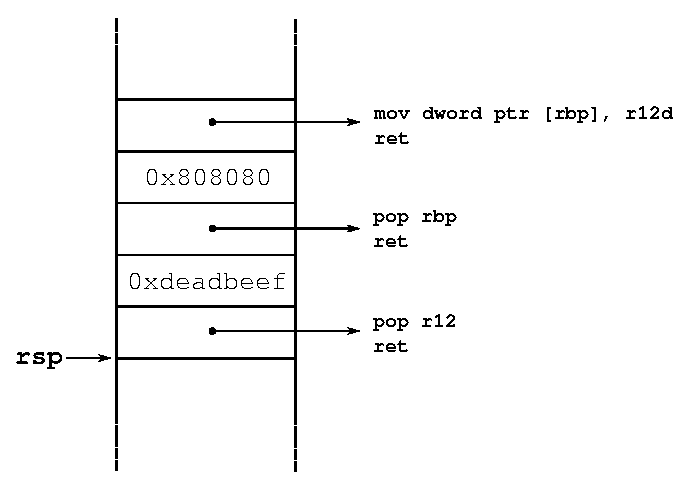
\includegraphics{rop}
\caption{Payload per la scrittura in memoria di una costante}
\label{fig:rop}
\end{figure}

In base all'eseguibile che stiamo considerando però potrebbero non
essere disponibili gadget esattamente come questi.  In particolare
potrebbero presentarsi altre istruzioni tra quella che a noi
effettivamente interessa (perché svolge la funzione a noi ``utile'') e
l'istruzione \lstinline{ret}. A volte modificando opportunamente lo
stack si può fare in modo che gli effetti di queste istruzioni non
incidano sulla nostra computazione. Ovviamente altri gadget, o
sequenze di gadget, possono svolgere funzioni equivalenti e, il fatto
che una categoria di gadget non è disponibile non implica che la
stessa funzione non possa essere svolta utilizzando gadget e/o
strategie differenti. Ad esempio se non abbiamo a disposizione un
gadget che ci permetta di impostare il registro \lstinline{eax}
tramite \lstinline{pop eax;ret} un'opportuna combinazione di
\lstinline{mov eax, 0xFFFFFFFF;ret} e \lstinline{inc eax;ret} ci
permette (non considerando restrizioni sulla lunghezza del payload) di
impostare valori arbitrari in \lstinline{eax}. Estrapolare, in maniera
automatica, sequenze e combinazioni di gadget che ci permettano di
raggiungere condizioni desiderate gestendo gli effetti secondari delle
istruzioni ``superflue'' rappresenta la parte più impegnativa
dell'implementazione di Dropper.

Le operazioni che l'architettura ci permette di eseguire non si
limitano ad operazioni di lettura e scrittura. Infatti possiamo
eseguire operazioni aritmetiche, operazioni logiche e utilizzare
sequenze di gadget che ci permettono di controllare il flusso del
programma. Come considerato nel paragrafo precedente spesso i metodi
per eseguire queste operazioni non sono diretti, ma è necessario
considerare gli effetti secondari e operare solo con i gadget a
disposizione. Ad esempio possiamo avere a disposizione solo operazioni
che operano su dimensioni di un byte, e per eseguire operazioni su
dimensioni maggiori è necessario concatenare più volte la stessa
operazione eseguendola un byte per volta, oppure un'operazione
potrebbe essere eseguita utilizzando una serie di più operazioni ma
che nel complesso sia equivalenti all'operazione voluta.

\subsection{Address Space Layout Randomization}

L'\emph{'Address Space Layout Randomization} (ASLR) è una tecnica di
protezione che consiste nel caricare in posizione casuale regioni
della memoria del programma. Questo è possibile perché un'istruzione
può riferirsi ad una locazione di memoria tramite la distanza tra il
proprio indirizzo (contenuta nel registro instruction pointer) e la
locazione in esame. Non utilizzando quindi più indirizzi assoluti il
codice può risultare indipendente dalla posizione di memoria in cui è
caricato a patto che che gli offset relativi restino invariati (cioè
che il codice non venga ``mischiato''). Il dynamic linker e alcune
strutture dati vengono utilizzate per far funzionare porzioni di
codice indipendenti anche dagli offset relativi (come nel caso del
testo dell'eseguibile e le librerie dinamiche), utilizzando un livello
di indirezione (vedi sez. \ref{sec:plt} e \ref{sec:got}).

L'utilizzo dell'ASLR porta due complicazioni principali nell'utilizzo
di tecniche basate sulla ROP. Prima di tutto non conoscendo
l'indirizzo di una porzione di codice non si possono conoscere neanche
gli indirizzi dei gadget contenuti all'interno. Questo riduce
notevolmente la quantità di gadget a disposizione, e, a seconda di
quanto codice venga casualizzato può rendere impossibile un attacco
che utilizzi la ROP. Infatti anche se solitamente, per questioni di
efficienza, solo le librerie vengono casualizzate, è possibile
compilare un'eseguibile in modo che una volta eseguito tutte le aree
che contengono codice vengano casualizzate (\emph{Position Indipendent
  Executable} (PIE)). In quest'ultimo scenario, a meno di non ottenere
informazioni sulla posizione di memoria in altri modi (ad esempio
tramite altre vulnerabilità che espongano indirizzi di strutture
dell'eseguibile), l'applicazione della ROP non risulta possibile.

Inoltre a venire casualizzate non sono solo porzioni che contengono
codice, ma anche la porzione di memoria riservata allo stack. Non
conoscendo la posizione dello stack risulta molto più difficile creare
sequenze di gadget che possano eseguire operazioni di controllo del
flusso. Una possibile soluzione potrebbe essere quella di iniettare
gli indirizzi dei gadget in un'altra posizione (nota) e modificare il
valore del registro dello stack perché punti a quella zona di memoria,
ovvero creare un \emph{Fake Stack Frame}. In più non avendo più
accesso a librerie dinamiche come la libc, difficilmente si riesce a
trovare nella porzione di codice non casualizzato istruzioni che ci
consentano di lanciare una syscall (solitamente il programma fa
affidamento alla libreria C per eseguirle e quindi dovrebbe comparire
tra le sequenze di istruzioni non ``intenzionali''). Tuttavia in
\cite{schwartz-2011} è stato dimostrato come anche utilizzando gadget che si
incontrano in porzioni di codice relativamente piccole è possibile
eseguire computazioni arbitrarie, addirittura concatenando questi
gadget in maniera automatica. In più come vedremo nelle prossime
sottosezioni è possibile, sotto alcune condizioni, ricavare gli
indirizzi di funzioni presenti nella libc partendo dalle strutture
dati coinvolte nelle operazioni di dynamic linking. Se le giuste
tipologie di gadget sono disponibili è possibile quindi eseguire
comandi arbitrari (come lanciare una shell) anche in contesti in cui
stack e librerie sono casualuzzati.


\subsection{Return-to-plt, GOT dereferencing e GOT patching}
\label{sec:expl}

In questa sottosezione presupponiamo che il codice del testo
dell'eseguibile non sia stato casualizzato. Anche se le librerie sono
casualizzate se un'eseguibile utilizza una funzione presente in una
libreria dinamica il linker, in fase di building, inserisce un
elemento della PLT relativo a quella funzione (vedi
sez. \ref{sec:plt}). Se la posizione in cui viene caricato il codice è
nota lo è anche quella della PLT e quindi l'indirizzo
dell'elemento. Questo ci permette di poter ``utilizzare'' nella nostra
catena le funzioni che utilizza l'eseguibile bersaglio, dirottando il
flusso all'indirizzo del relativo elemento nella \lstinline{PLT}, da
qui il nome \emph{return-to-plt}. Una volta utilizzata una funzione il
valore dell'indirizzo assoluto di quella funzione si verrà a trovare
nell'elemento relativo nella GOT (vedi sez. \ref{sec:got}). Come
descritto in \cite{roglia:2009} questo ci permette di utilizzare due
tecniche di attacco particolari: \emph{GOT dereferencing} e \emph{GOT
  patching}. Tutte e due le tecniche utilizzano l'indirizzo assoluto
di una funzione contenuto nell'elemento relativo nella GOT per
calcolare l'indirizzo assoluto di una funzione della libc desiderata,
di fatto eludendo ASRL. Nella prima tecnica il valore viene letto,
modificato tramite un'operazione aritmetica e viene poi eseguito un
salto a questo indirizzo. Un esempio di gadget che consentono questo
tipo di attacco sono: \lstinline{add eax,[ebx+off];ret} e
\lstinline{jmp [eax]}. La seconda tecnica invece modifica l'elemento
della GOT in loco, utilizzando poi un return-to-plt per richiamare la
funzione voluta. Un esempio di gadget che può essere utilizzato per
modificare la funzione in loco è:

\lstinline{adc byte ptr [esi + 0x5f], bl ; pop ebp ; ret}

Infatti concatenando diverse istruzioni del genere insieme ad
opportuni gadget che impostarino i registri \lstinline{esi o ebx} è
possibile aggiungere un offset arbitrario in una locazione di memoria
arbitraria. È da notare che questa tecnica non funziona nel caso la
GOT sia in un'area di memoria non scrivibile (ad esempio se
l'eseguibile è stato compilato con l'opzione RELRO) ma i gadget
utilizzati in questa seconda tecnica sono di un tipo più comune
rispetto a quelli utilizzati nella GOT dereferencing.


%%% Local Variables: 
%%% mode: latex
%%% TeX-master: "tesi"
%%% End: 
